\chapter{Theoretical  Motivation}

In order to talk about my thesis work it will be necessary to dive into some of the theoretical
background motivating my results. Particle physics is a study of the fundamental building blocks
of the universe and is vast in its nature. I will try to elucidate some of the more pertinent points here. 
I will begin with a brief tour through the Standard Model (SM) followed by a more detailed explanation
the Higgs mechanism and electroweak symmetry breaking. This section was structurally inspired by the 
material in Modern Particle Physics by Mark Thomson, which served as a steady guide for me throughout 
my journey in graduate school.

\section{Fundamentals of the Standard Model}

The Standard Model (SM) is a quantum field theory describing all known fundamental particles and 
their interactions through 3 out of the 4 known fundamental forces: the electromagnetic (EM) force, the 
weak nuclear force and the strong nuclear force. It combines our understanding of quantum mechanics and 
special relativity, providing a comprehensive but not completely unified prescription of particle physics 
due to its missing incorporation of general relativity (and thus gravity). The Standard Model 
is defined by its gauge symmetry group $SU(3)\times SU(2)\times U(1)$, which describes a local mathematical 
transformation that leaves a particular system invariant. This symmetry is deeply linked with the 
appearance of the three forces incorporated in the SM. In particular, $SU(3)$ is associated with the strong 
nuclear force while $SU(2)\times U(1)$ describes the unified electroweak interaction. The latter symmetry is 
spontaneously broken by the Higgs mechanism, leading to the separate manifestation of the weak and 
EM forces in nature. \par

\subsection{Particles of the Standard Model}

The particles in the SM are broadly grouped into two categories based on their spin: fermions have half-
integer spin and obey Fermi-Dirac statistics while bosons have integer spin and obey Bose-Einstein 
statistics. All fundamental fermions in the SM have spin-$\textonehalf$ and are further categorized as quarks 
and leptons, which make up the matter particles. In addition, SM fermions come in 3 generations, which consist 
of one up-type quark ($q=\frac{1}{3}$), one down-type quark ($q=-\frac{2}{3}$), one charged lepton 
($q=1$) and one neutrino ($q=0$) each. Particles in successive generations differ only in their masses, 
making second and third generation fermions inherently unstable. This is the reason why most ordinary 
matter in the universe is made up of up-quarks, down-quarks and electrons rather than charm-quarks, 
strange-quarks and muons or top-quarks, bottom-quarks and taus. Quarks have a property called 
color charge associated with the $SU(3)$ symmetry (in addition to their EM charge),  which distinguishes 
them from leptons and enables them to interact via the strong force. Leptons do not share this property 
and thus only experience EM and weak interactions. Finally, each fermion has an anti-particle 
counterpart with identical characteristics, but opposite EM charge. Since neutrinos are charge neutral, their 
anti-particles are distinguished by their allowed interactions, although it is not yet clear whether neutrinos 
are their own anti-particles.\par

Bosons in the SM are split into four types of vector bosons (with spin $s=1$) and one scalar boson (with 
spin $s=0$), the Higgs. Vector bosons are force mediators generated by the symmetry groups of 
the SM. Gluons are associated with the strong force and come in 8 configurations of color charge 
(associated with the 8 generators of $SU(3)$). Due to the aforementioned symmetry breaking of 
$SU(2)\times U(1)$ associated with the separation of the weak and EM forces, the photon and $W$ and $Z$ 
bosons do not map quite as neatly onto the generators of this group. In practice, the photon is associated 
with the EM interaction while the massive $W$ and $Z$ bosons propagate the weak interaction. The 
observation that the mediators of the weak interaction are not massless lead to the introduction of a 
corrective mechanism to the SM which will be described in detail in a later section. This is the theoretical 
origin of the final particle in the SM which is the protagonist of this thesis, the Higgs boson. The only known 
fundamental scalar particle is deeply connected to the existence of particle masses and is, for now, probably 
the least understood aspect of the Standard Model of particle physics. \par

%https://www.researchgate.net/figure/The-Standard-Model-of-particle-physics-3_fig1_381551014
\begin{figure}
\centering
    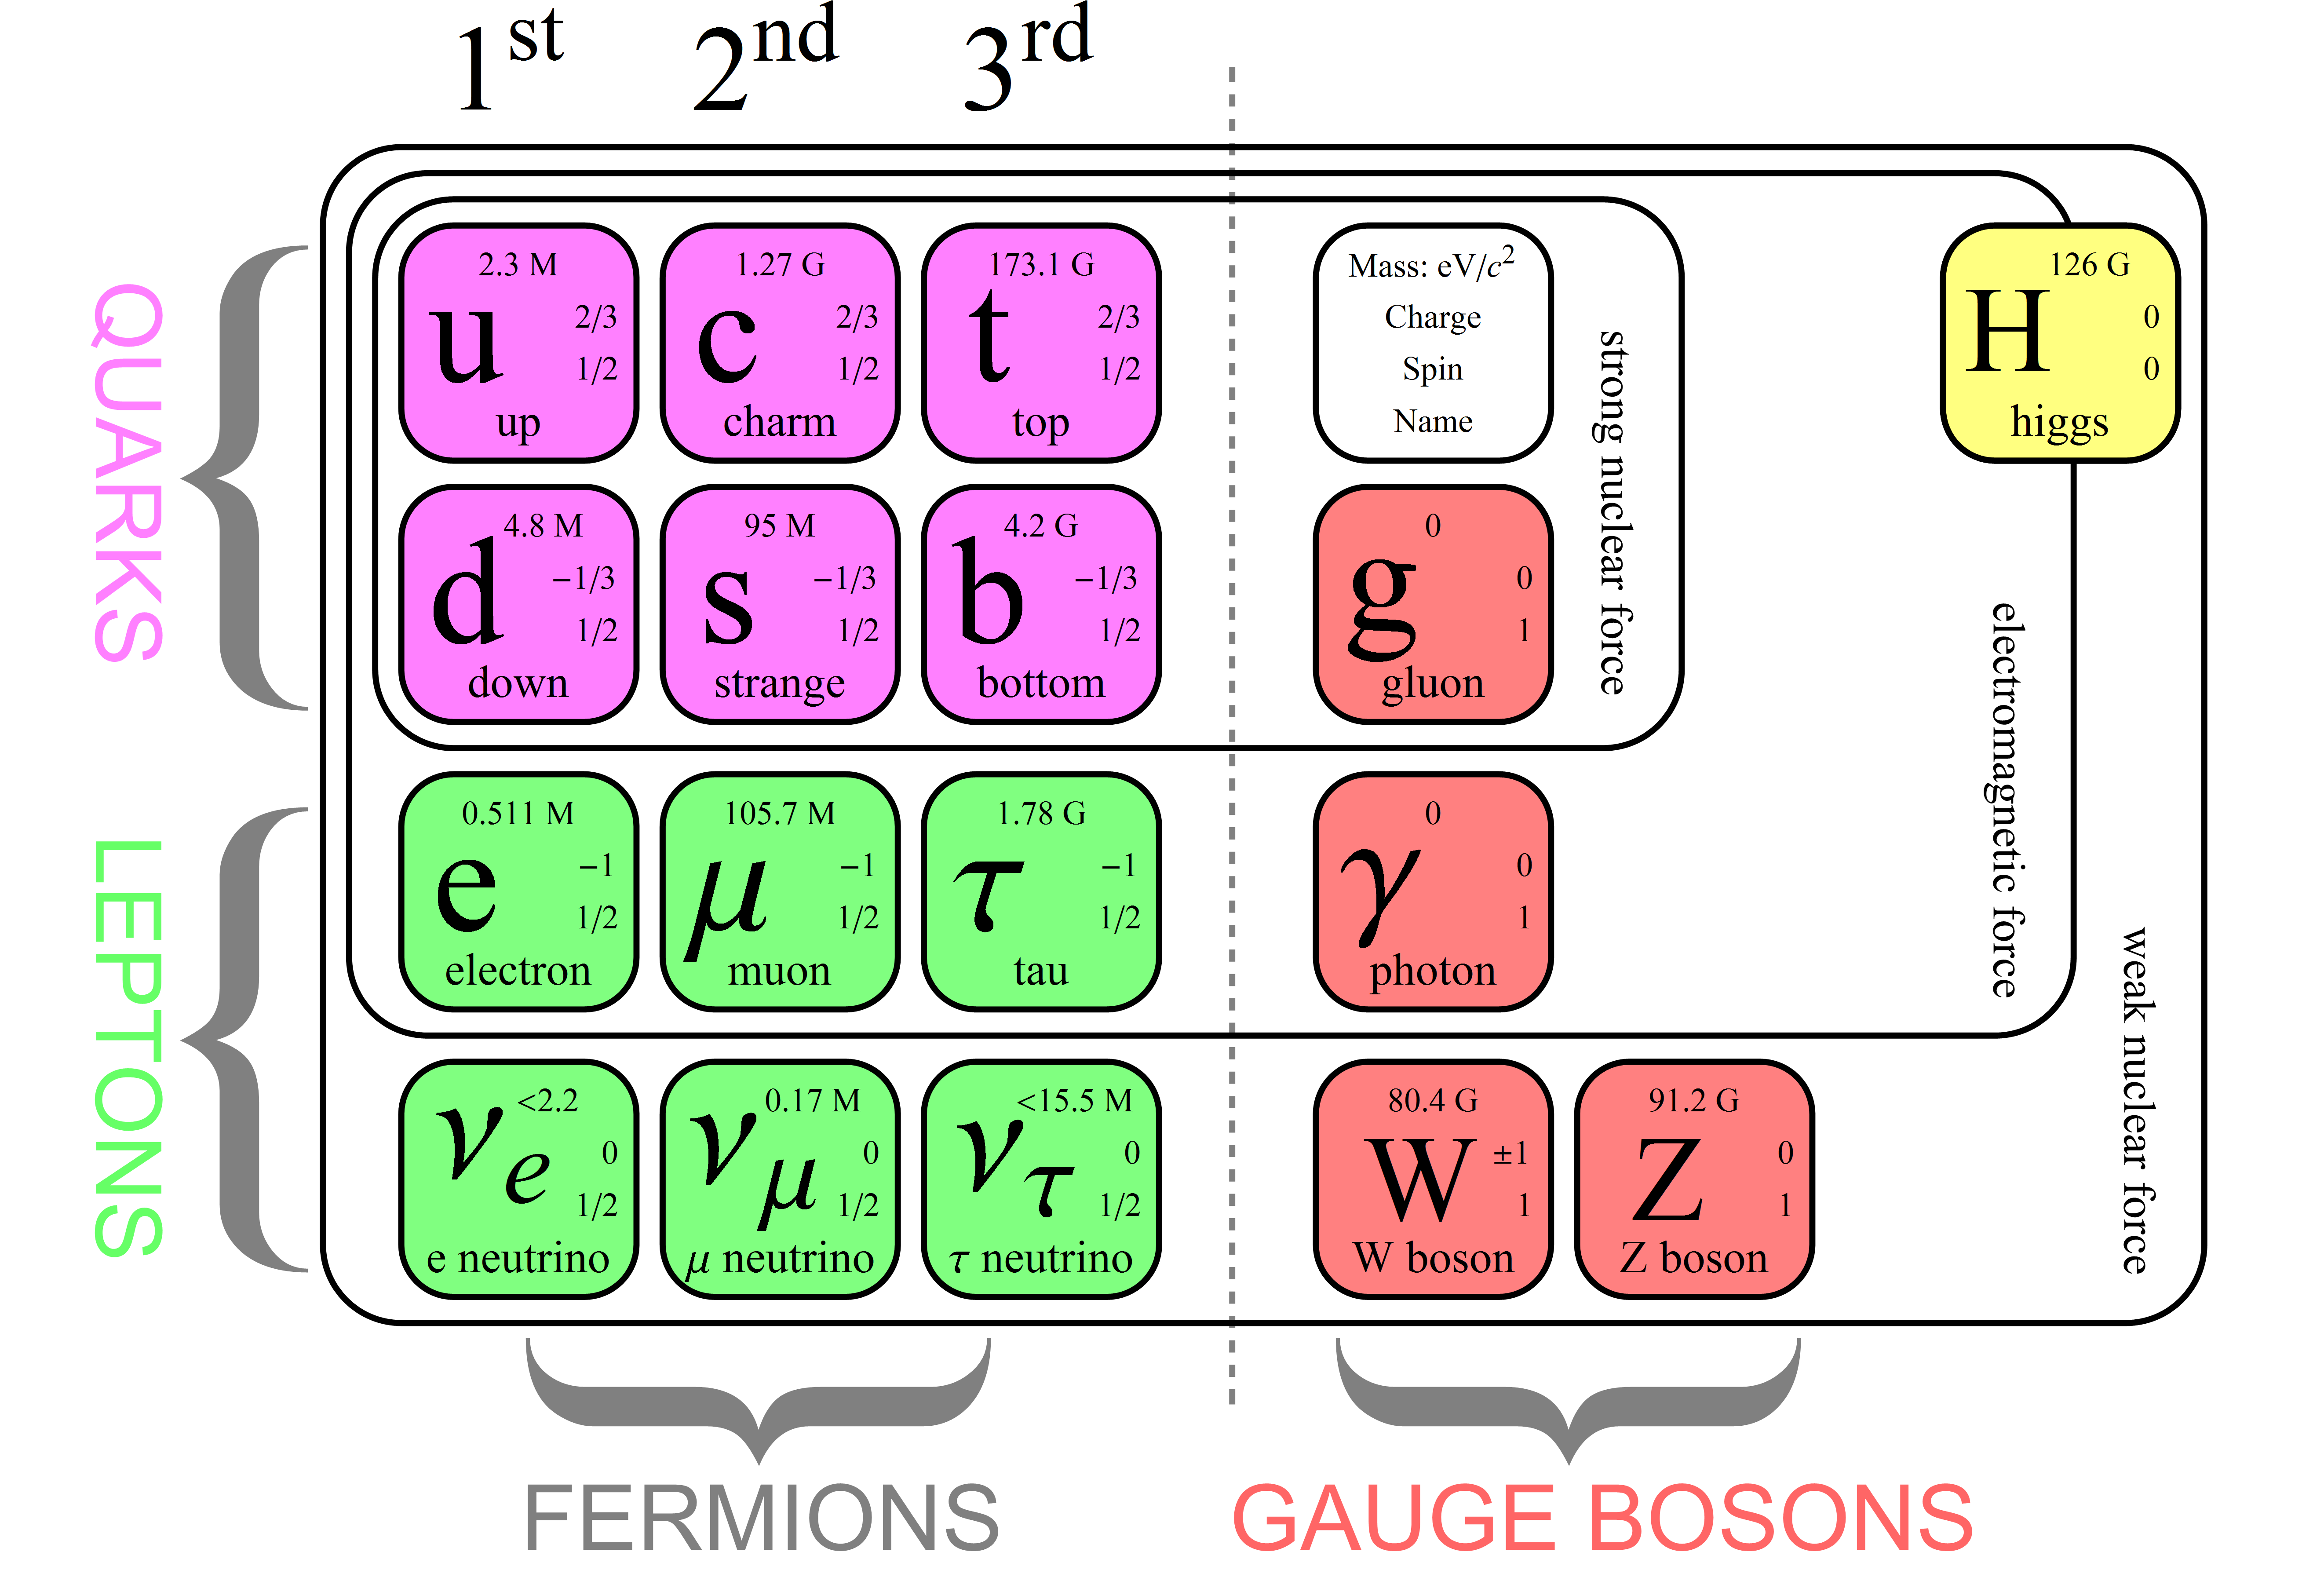
\includegraphics[width=0.8\textwidth]{images/Standard_Model.png}
    \caption{Graphical summary of Standard Model particles.}
    \label{fig:Standard_Model}
\end{figure}

\subsection{Mathematical Formalism}

In order to fully explore the significance of the Higgs boson, a tour through the mathematical formalism of the 
SM is necessary. As a quantum field theory, the fundamental objects of the SM are quantum fields (represented 
by spinors) whose excitations correspond to observable particles. Its Lagrangian $\mathcal{L}_{SM}$ is defined 
by some underlying symmetries, which consist of a global CPT-symmetry in addition to the 
$SU(3)\times SU(2)\times U(1)$ local gauge symmetries discussed above. CPT is a combination of charge 
conjugation (exchange of particles with anti-particles), parity (reversal of space) and time reversal. These three 
symmetries do not always hold individually within the SM (as we will explore), but their combination must always 
remain unbroken. \par

Mathematically, fermions are represented by Dirac spinors $\psi$ which have 4 independent components. 
These can be decomposed into two orthogonal two-component spinors $\psi_L = \frac{1}{2}(1-\gamma_5)\psi$ 
and $\psi_R = \frac{1}{2}(1+\gamma_5)\psi$ which represent chiral eigenstates that are related to each other 
via a parity transformation. This particular decomposition is important because these eigenstates (left-handed 
and right-handed spinors) are treated differently within some SM interactions (leading to violation of 
parity-symmetry). Each chiral spinor has a spin-up and a spin-down component. In the free particle case, a 
fermion field satisfies the Dirac equation 
\begin{equation}
(i\slashed{\partial} - m)\psi = 0
\end{equation}
where $\slashed{\partial} = (i\gamma^{\mu}\partial_{\mu} - m)$. Given $\bar{\psi} = \psi^{\dag}\gamma_0$, 
the free particle Lagrangian then consists simply of a kinetic term and a mass term
\begin{equation}
\mathcal{L} = i\bar{\psi}\gamma^{\mu}\partial_{\mu}\psi - m\bar{\psi}\psi
\end{equation}
This simple picture is complicated significantly by the presence of boson fields, which are responsible for 
introducing particle interactions described by Quantum Electrodynamics (QED), Quantum Chromodynamics 
(QCD), electroweak theory and the Higgs mechanism. Each of these aspects of the SM comes out of a particular 
gauge symmetry (or the breaking thereof), which are explored in the following sections.

\subsection{Quantum Electrodynamics (QED)}

QED postulates that the SM Lagrangian is invariant under a $U(1)$ local phase transformation of the form 
\begin{equation}
\psi(x) \rightarrow \psi'(x) = e^{iq\chi(x)}\psi(x)
\end{equation}
This symmetry is enforced in the Lagrangian with the introduction of the covariant derivative 
$D_{\mu} = \partial_{\mu} + iqA_{mu}$, where $A_{\mu} \rightarrow A_{\mu}' = A_{\mu} + \partial_{\mu}\chi(x)$. 
The Dirac Lagrangian is thus left invariant under the $U(1)$ transformation with the introduction of a new 
field $A_{\mu}$, which is coupled via the electric charge $q$ (and represents the photon). The choice of $\chi(x)$ 
is arbitrary and leads to the ability to define different gauges, allowing for some redundancy in the field 
description of electrodynamics. This means that the $U(1)$ symmetry manifests in practice via the exchange 
of photons between charged particles, described in full by the QED Lagrangian
\begin{equation}
\mathcal{L}_{QED} = - \frac{1}{4}F_{\mu\nu}F^{\mu\nu} + i\bar{\psi}\gamma^{\mu}D_{\mu}\psi - m\bar{\psi}\psi =
- \frac{1}{4}F_{\mu\nu}F^{\mu\nu} + i\bar{\psi}\gamma^{\mu}\partial_{\mu}\psi - q\bar{\psi}\gamma^{\mu}A_{\mu}\psi - m\bar{\psi}\psi
\end{equation}
Here $F_{\mu\nu} = \partial_{\mu}A_{\nu}  - \partial_{\nu}A_{\mu}$ is just the field strength tensor that represents 
the kinetic term of the photon, which describes the propagation of electromagnetic fields. The covariant derivative 
brings out both the standard kinetic term for fermions, as well as a fermion-photon interaction term which is only 
present when $q \neq 0$ as expected.  This means that photons do not interact with neutral fermions.

\subsection{Quantum Chromodynamics (QCD)}

From the comparatively simple symmetry underlying QED we can now move towards of a description 
of the more complicated theory of Quantum Chromodynamics (or QCD), which aims to explain the strong nuclear 
interaction.  As in QED, this theory is described by a local gauge symmetry, which in this case is an $SU(3)$ symmetry 
enforcing invariance under transformations of the form
\begin{equation}
\psi(x) \rightarrow \psi'(x) = exp[ig_{S} \boldsymbol{\alpha}(x) \cdot \boldsymbol{\hat{T}}] \psi(x)
\end{equation}
Here $\boldsymbol{\hat{T}} =  \{T^a\}$ are the 8 generators of the $SU(3)$ group and $\boldsymbol{\alpha}(x)$ is 
a set of 8 arbitrary functions. Each generator of $SU(3)$ is represented by a 3x3 matrix, requiring the addition of 
three extra degrees of freedom to the description of the fermionic wavefunction $\psi(x)$.  The orthogonal states in 
this new three-dimensional space are the three color eigenstates red, green and blue. All quarks carry a color charge 
while antiquarks carry an anticolor charge and the combination of a matching color and anticolor charge (e.g. blue and 
anti-blue) is colorless.  Strong interactions occur via the exchange of gluons, which carry one color and one anticolor 
charge. There are 8 gluons total, corresponding to the 8 generators of $SU(3)$. The analogy between QCD and QED can 
be seen directly in the QCD Lagrangian
\begin{equation}
\mathcal{L}_{QED} = 
%- \frac{1}{4}G^a_{\mu\nu}G^{\mu\nu}_a + i\bar{\psi_i}\gamma^{\mu}(D_{\mu})_{ij}\psi_j - m\bar{\psi_i}\delta_{ij}\psi_j =
- \frac{1}{4}G^a_{\mu\nu}G^{\mu\nu}_a + i\bar{\psi_i}\gamma^{\mu}\partial_{\mu}\delta_{ij}\psi_j +g\bar{\psi_i}\gamma^{\mu}(T_a)_{ij}\mathcal{A}^a_{\mu}\psi_j  - m\bar{\psi_i}\delta_{ij}\psi_j
\end{equation}
As can be seen, the gluon exchange term, which contains the gluon fields $\mathcal{A}^a_{\mu}$, is the only term that 
can mix different color components of the wavefunction $\psi$. The gluon field strength tensor $G^a_{\mu\nu} = 
\partial_{\mu}\mathcal{A}^a_{\nu} - \partial_{\nu}\mathcal{A}^a_{\mu} + 
gf^{abc}\mathcal{A}^b_{\mu}\mathcal{A}^c_{\nu}$ replaces the electromagnetic field strength tensor to form the 
kinetic term of the fields. \par

A unique aspect of QCD is the requirement that free particles exist in colorless states. This is called color confinement 
and prevents quarks from existing outside of bound states such as baryons ($qqq$) or mesons ($q\bar{q}$). While an 
analytical proof of this mechanism does not exist, it can be understood through the fact that the energy stored in the 
field between two separated quarks grows linearly with the separation distance $V(r) ~ \kappa r$ (with $\kappa ~ 
1 GeV/fm$). This stands in stark contrast to the $\frac{1}{r}$ potential in electrodynamics which allows for the 
existence of free electric charge. Color confinement has wide-ranging implications for collider physics which will be 
discussed in detail in later sections.

\section{The Electroweak Sector}

The theories of Quantum Electrodynamics and Quantum Chromodynamics are structured mostly identically, up to their 
unique symmetry groups that give rise to their respective exchange particles and conserved quantities. The weak 
interaction follows a similar, but not identical blueprint. Among its peculiarities are its three massive exchange bosons 
($W^{\pm}$ in charged-current and $Z$ in neutral-current interactions) as well as its unique ability to violate the 
combined symmetries of charge conjugation and parity (CP). It is also intricately linked to the electromagnetic 
interaction via the manifestation of a combined $SU(2) \times U(1)$ symmetry in the Standard Model. This symmetry, 
or rather the breaking thereof, is key to understanding the role of the Higgs boson in particle physics. 

\subsection{The Charged Current}

The charged-current weak interaction occurs via the exchange of charged $W^{\pm}$ bosons and was first 
studied in nuclear beta decay, where its parity violating properties were observed. Examining beta decays in an 
applied magnetic field showed a preferred direction for the emission of the electron relative to the B field, 
suggesting that the weak interaction maximally violates parity. This stands in stark contrast to both QED and QCD 
interactions whose Lagrangians have interaction terms with Lorentz covariant currents of the form
$j^{\mu} = \bar{u}(p')\gamma^{\mu}u(p)$, which transform as four-vectors and are thereby inherently parity 
conserving. While the QED and QCD currents both transform as four-vectors in practice, assuming Lorentz covariance 
there is nothing preventing other kinds of interactions that transform as scalars, pseudoscalars, axial vectors or 
tensors (with the rank of each corresponding to the spin of the hypothetical exchange boson). Thus is natural to 
assume that the charged weak current does not transform as a vector, but rather an axial vector (since we know 
its exchange boson is a vector boson with spin 1). This would suggest a current of the form 
$\bar{\psi}\gamma^{\mu}\gamma^{5}\phi$. In reality, for parity violation to take place we require a current with both 
vector and axial vector components. For the weak interaction this current is
$j^{\mu} = \frac{g_W}{\sqrt{2}}\bar{u}(p')\frac{1}{2}\gamma^{\mu}(1-\gamma^{5})u(p)$, which is a maximally parity 
violating V-A (i.e. vector - axial vector) interaction. Notably, this term contains the left-handed chiral projection 
operator which projects out right-handed components of particle wavefunctions. As such,  the charged-current weak 
interaction can only occur between left-handed particles (or right-handed anti-particles). \par

Putting this interaction into the same language as the discussions of QED and QCD, it is associated with an invariance 
under local $SU(2)$ phase transformations for left-handed particles (and right-handed anti-particles) only. This is 
denoted $SU(2)_L$ and takes the form 
\begin{equation}
\psi(x) \rightarrow \psi'(x) = exp[ig_{W} \boldsymbol{\alpha}(x) \cdot \boldsymbol{\hat{T}}] \psi(x)
\end{equation}
where this time $\boldsymbol{\hat{T}} = \frac{1}{2}\boldsymbol{\sigma}$ are the three generators of the SU(2) 
group (i.e. the Pauli spin matrices). The new interaction terms in the Lagrangian that come from this symmetry are 
just $ig_W\frac{1}{2}\sigma_k\gamma^{\mu}W_{mu}^k\psi_L$, where the physical $W^{\pm}$ bosons are linear 
combinations of $W^{(1)}$ and $W^{(2)}$ given by 
$W^{\pm}_{\mu} = \frac{1}{\sqrt{2}}(W^{(1)}_{\mu} \mp iW^{(2)}_{\mu})$ and the $W^(3)$ is related to the 
neutral-current discussed in section X. Due to the 2x2 nature of the generators of $SU(2)$, $\psi_L$ must consist 
of two components making up a doublet (analogous to the color triplet in QCD). In this case, the two states of this 
doublet represent different physical particles (separated by one unit of charge) which are connected via a 
conserved quantity called weak isospin. The exchange of a $W^{\pm}$ boson allows the system to transition 
between these two states. This means that left-handed particles are represented as
\begin{equation}
\begin{pmatrix} \nu_{l} \\ l^- \end{pmatrix}_L, 
\begin{pmatrix} u \\ d' \end{pmatrix}_L
\end{equation}
while right-handed particles are placed in $SU(2)_L$ invariant weak isospin singlets, thereby linking left-handed 
neutrinos and charged leptons as well as up-type and down-type quarks via the charged current weak interaction.  
The $d'$ in the above description does not represent a pure down quark state but rather a combination of down-type 
quark states with marginal contributions from strange and bottom quarks.

\subsection{CP Violation and the CKM Matrix}

The details of how the charged-current weak interaction manifests differs in practice between leptons and quarks. In 
leptons, $W^{\pm}$ exchange allows for interactions between charged leptons and their corresponding neutrinos. Lepton 
flavor needs to be conserved in these interactions, so electron neutrinos only interact with electrons, muon neutrinos with 
muons and tau neutrinos with taus. The strength of each of these is identical, captured in a concept called lepton universality in weak interactions. While parity and charge conjugation are maximally violated as individual symmetries 
due to the left-handedness of the weak interaction, the leptonic charged-current conserves CP symmetry. In general, CP 
violation involving leptons only occurs due to the properties of neutrinos themselves, which will be discussed in section 
X. \par

Taking this into account, the possibility for CP violation in weak interactions must therefore come from the quark sector. 
In particular, attempts to extend lepton universality into a universal weak coupling for quarks and leptons proved 
unfruitful as differences in interaction strengths between leptonic and hadronic weak interactions were observed. 
This observation also extended to different kinds of hadronic interactions, leading to the formulation of the Cabibbo 
hypothesis which states that the mass eigenstates of quarks are not equal to their weak eigenstates. A universal 
coupling therefore exists when considering the weak eigenstates $q'$, which are related to the mass eigenstates $q$ 
via the CKM matrix
\begin{equation}
\begin{pmatrix} d'  \\ s' \\ b' \end{pmatrix} =
\begin{pmatrix} V_{ud} & V_{us} & V_{ub} \\ V_{cd} & V_{cs} & V_{cb} \\ V_{td} & V_{ts} & V_{tb} \end{pmatrix}
\begin{pmatrix} d \\ s \\ b \end{pmatrix}
\end{equation}
The nine elements of this matrix can be parametrized via three rotation angles and a complex phase because of 
unitarity conditions. The misalignment of quark eigenstates leads to observable instances of CP violation in weak 
interactions involving quarks, which is one of the main known sources of CP violation within the Standard Model. The 
CKM matrix itself has been studied thoroughly via experiments, with the most recent constraints showing off diagonal 
elements to be relatively small in general. This is particularly true for the top quark which essentially exclusively decays 
to bottom rather than strange or down.

\subsection{Electroweak Unification}

The local $SU(2)_L$ symmetry of the weak interaction has three generators, implying three conserved currents and thus 
three exchange particles. Thus far we have thoroughly discussed the first two,  $j_+$ and $j_-$ corresponding to the 
$W^{\pm}$ bosons which mediate the charged-current weak interaction. We will now explore the third current, $j_3$, 
which is related to the neutral-current interactions mediated by the $Z$ boson.  \par

In a universe where $j_3$ corresponds to the exchange of a $Z$ boson, we expect right-handed particles (and 
left-handed anti-particles) to not participate in these interactions due to the fixed handedness of the $SU(2)_L$ 
symmetry. Upon investigation however, we find that this is empirically not true: the $Z$ boson interacts with particles 
regardless of handedness, albeit slightly unevenly. This complicates our description of the weak interaction significantly, 
requiring a modification of our presumed symmetry. In practice, we need to modify and integrate the fundamental 
$U(1)$ symmetry of electromagnetism with the $SU(2)_L$ symmetry of the weak interaction. For this to work, the 
$U(1)$ symmetry cannot couple to electric charge as discussed in section X, but rather a new quantity called weak 
hypercharge $Y$. The resulting interaction term $g'\frac{Y}{2}\gamma^{\mu}B_{\mu}\psi$ is analogous to QED with 
an altered coupling and replacement of the photon field $A_{\mu}$ by $B_{\mu}$. The actual photon and Z boson 
fields
\begin{equation}
A_{\mu} = B_{\mu}cos\theta_W + W^{(3)}_{\mu}sin\theta_W
\end{equation}
\begin{equation}
Z_{\mu} = -B_{\mu}sin\theta_W+W^{(3)}_{\mu}cos\theta_W
\end{equation}
are then taken to be linear combinations of the $U(1)_Y$ field and the neutral $SU(2)_L$ field with the weak mixing 
angle $\theta_W$ characterizing the strength of the mixing. The electron charge is related to the $U(1)_Y$ and 
$SU(2)_L$ couplings as well as the mixing angle by $e = g_Wsin\theta_W = g'cos\theta_W$. Putting all of this 
together we now have a theory with a combined electroweak symmetry given by $SU(2)_L \times U(1)$. While 
this provides a unified description of electromagnetism and weak sector physics, there is a fundamental issue with our 
description of particle physics: particle mass is unaccounted for.

\section{The Higgs Boson}

All symmetries of the Standard Model discussed thus far require that each term in the Lagrangian 
$\mathcal{L}_{SM}$ of our complete theory be invariant under $U(1)$, $SU(2)_L$ and $SU(3)$ local gauge 
transformations. The QED, QCD and weak components of $\mathcal{L}_{SM}$ are constructed with these symmetries 
in mind, but each only contain kinematic and interaction terms between fermions and exchange bosons. To enforce 
the existence of particle masses we need to introduce self-interaction terms for all massive particles, which are of the 
form $\frac{1}{2}m_V^2V_{\mu}V^{\mu}$ for bosons and $m_f\bar{f}f = m_f(\bar{f}_Rf_L + \bar{f}_Lf_R)$ for 
fermions. All of these additional terms are fundamentally incompatible with the prescribed symmetries of the Standard 
Model since they are not invariant under $SU(2)_L \times U(1)_Y$ transformations. This means that without further 
modifications, the Standard Model is incompatible with the existence of massive particles, which is (of course) 
empirically hard to justify given our understanding of the physical universe. Fixing this requires the introduction of a 
scalar boson (the Higgs) and the breaking of our $SU(2)_L \times U(1)_Y$ symmetry, which will be discussed in the 
following sections.

\subsection{Scalar fields and symmetry breaking}

The origin of particle mass terms in the Lagrangian of the Standard Model lies in a process known as spontaneous 
symmetry breaking which occurs in the electroweak sector of our theory. The backbone of this is the introduction of 
a new complex scalar field $\phi$ (which we will identify as the Higgs field) with a Lagrangian of the form 
$(D_{\mu}\phi)^*(D^{\mu}\phi) - V(\phi)$ where $V(\phi) = \mu^2\phi^2 + \lambda\phi^4$ is the Higgs potential 
and $D_{\mu}$ represents the covariant derivative (which enforces gauge invariance as in the QED and QCD 
Lagrangians). For a single complex scalar field $\phi = \frac{1}{\sqrt{2}}(\phi_1 + i\phi_2)$ the potential expands to
\begin{equation}
V(\phi) = \frac{1}{2}\mu^2(\phi_1^2 + \phi_2^2) - \frac{1}{4}\lambda(\phi_1^2 + \phi_2^2)^2
\end{equation}
where we require $\lambda > 0$ to ensure the potential has a finite minimum. The choice of $\mu$ then determines 
the shape of the potential, with $\mu^2 > 0$ leading to a minimum at 0 and $\mu^2 < 0$ to a set of minima defined 
by $\phi_1^2 + \phi_2^2 = -\frac{\mu^2}{\lambda}$, as shown in Figure \ref{fig:Higgs_Potential}. 

\begin{figure}
\centering
    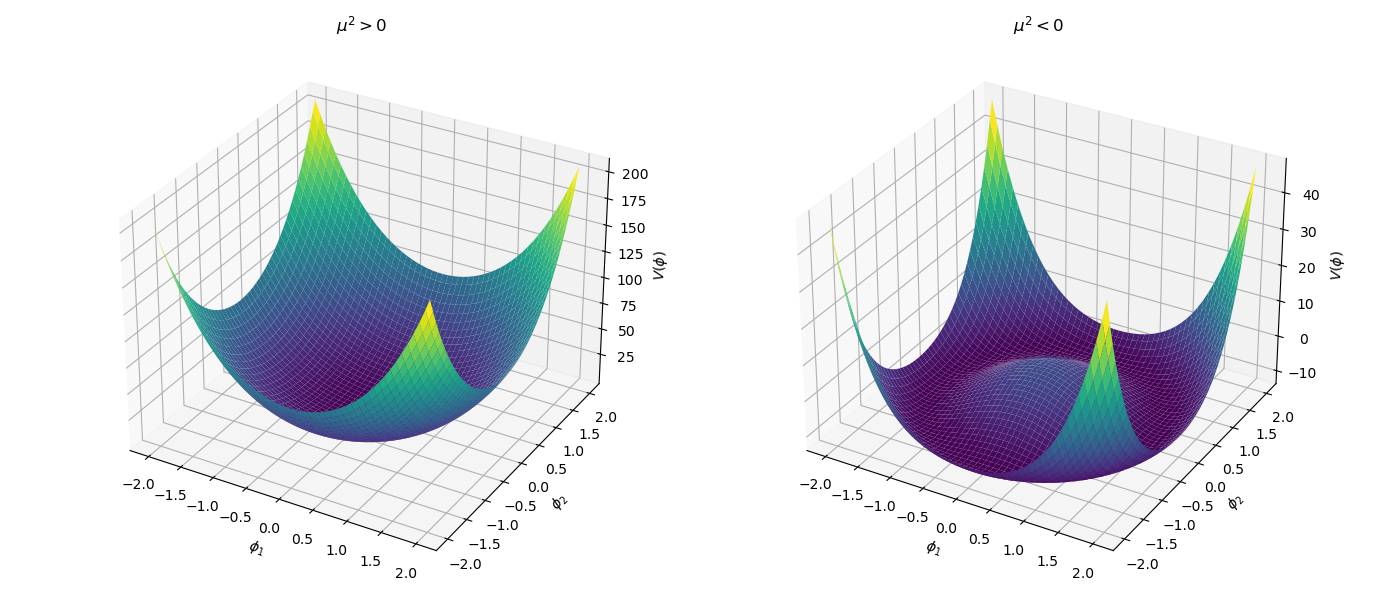
\includegraphics[width=1.0\textwidth]{images/Higgs_Potential.png}
    \caption{Visual representation of the Higgs potential (with $\lambda = 2$) for positive $\mu^2 = 10$ (left) and 
    negative $\mu^2 = -10$ (right).}
    \label{fig:Higgs Potential}
\end{figure}

In the case where $\mu^2 < 0$, this potential requires a physical choice for the minimum (vacuum) state which 
explicitly breaks the rotational symmetry in the $(\phi_1, \phi_2)$ plane. The minimum energy of the system, also 
known as the vacuum expectation value (or VEV), is at $v = \sqrt{\frac{-\mu^2}{\lambda}}$ for such a theory. \par

In the Standard Model we require the scalar field to be a complex $SU(2)$ doublet
\begin{equation}
\phi = 
\begin{pmatrix} \phi^+  \\ \phi^0 \end{pmatrix}
= \frac{1}{\sqrt{2}}
\begin{pmatrix} \phi_1 + i\phi_2 \\ \phi_3 + i\phi_4 \end{pmatrix}
\end{equation}
which given $\mu^2 < 0$ has an infinite number of minima where $\phi^\dagger\phi = \frac{v^2}{2}$. For physical 
reasons related to the absence of photon mass, the vacuum expectation value is only non-zero for the $\phi^0$ 
component of the doublet, such that we can expand the field around this minimum as
\begin{equation}
\phi(x) = \frac{1}{\sqrt{2}}
\begin{pmatrix} 0 \\ v + h(x) \end{pmatrix}
\end{equation}
This field description is in unitary gague where $h(x)$ directly represents the physical Higgs field. An equivalent, 
but more general description of this expansion around the VEV can be done by including an additional perturbing 
field around the minimum of $\phi^+$ and then removing non-physical fields via gauge transformation afterwards. 
In the end, the symmetry breaking of this new scalar potential immediately results in the introduction of weak
boson mass terms in the Lagrangian as well as an entirely new particle: the Higgs boson.

\subsection{Particle masses and Higgs interactions}

The origin of weak boson masses can be seen directly if we expand the kinetic term of the scalar field 
Lagrangian around the VEV as
\begin{equation}
\begin{aligned}
(D_{\mu}\phi)^{\dagger}(D^{\mu}\phi) =& \frac{1}{2}(\partial_{\mu}h)(\partial^{\mu}h) + 
\frac{1}{8}g_W^2(W_{\mu}^{(1)} + iW_{\mu}^{(2)})(W^{(1)\mu} - iW^{(2)\mu}(v+h)^2 + \\
&\frac{1}{8}(g_WW_{\mu}^{(3)} - g'B_{\mu})(g_WW^{(3)\mu} - g'B^{\mu})(v+h)^2 \\
=&\frac{1}{2}(\partial_{\mu}h)(\partial^{\mu}h) + \frac{1}{4}g_W^2W_{\mu}^-W^{+\mu}(v+h)^2 + 
\frac{1}{4}(g_W^2+g'^2)Z_{\mu}Z^{\mu}(v+h)^2
\end{aligned}
\end{equation}
where we have written the physical particles as combinations of the underlying fields 
$W^{\pm} = \frac{1}{\sqrt{2}}(W^{(1)} \mp iW^{(2)})$ and 
$Z = (g^2_W + g'^2)^{-\frac{1}{2}}(g_WW^{(3)} - g'B)$. In this expression,  the $v^2$ terms represent 
the weak boson masses (i.e. self-interaction terms) while $vh$ and $h^2$ terms describe the couplings 
(i.e. interaction strengths) between two weak bosons and one or two Higgs bosons respectively. The masses 
can be read directly from the Lagrangian as $m_W = \frac{1}{2}g_Wv$ and 
$m_Z = \frac{1}{2}v\sqrt{g^2_W + g'^2}$. As expected, there is no mass term for the photon, which means 
it does not interact with the Higgs boson. Requiring orthogonality to the $Z$, we can see that the photon is 
represented as $A = (g^2_W + g'^2)^{-\frac{1}{2}}(g'W^{(3)} + g_WB)$. Repeating the above expansion 
with the potential term of the scalar field Lagrangian results in 
\begin{equation}
V(\phi) = \frac{1}{2}\mu^2(v+h)^2 + \frac{1}{4}\lambda(v+h)^4 = 
\lambda v^2h^2 + \lambda vh^3 + \frac{1}{4}\lambda h^4 - \frac{1}{4}\lambda v^4
\end{equation}
where $h^2$ terms define the Higgs mass $m_H = \sqrt{2\lambda}v$ and $h^3$ and $h^4$ terms the 
self-couplings between 3 and 4 Higgs bosons respectively. \par

These new additions to the Standard Model Lagrangian bring out the missing mass terms for weak bosons 
via the introduction of a massive scalar boson: the Higgs. Fermions on the other hand, are still unaccounted 
for.Thankfully, the Higgs field allows for the introduction of gauge invariant fermion mass terms which 
complete the picture. In particular these take the form of 
$-g_f(\bar{\psi_L}\phi\psi_R + \bar{\psi_R}\phi^{\dagger}\psi_L$ and 
$g_f(\bar{\psi_L}\phi_C\psi_R + \bar{\psi_R}\phi_C^{\dagger}\psi_L$, which satisfy the 
$SU(2)_L \times U(1)_Y$ symmetry of the Standard Model.

\section{Why the Higgs is interesting}

While the Standard Model is mathematically robust and broadly experimentally tested, there are still open 
questions about elements of its Lagrangian. It has 19 free parameters that are not fixed by theoretical 
predictions. Of these, 9 are related to the masses of the quarks and charged leptons, 4 to the CKM 
matrix (3 angles + 1 phase), 3 are coupling strengths, 2 are related to the Higgs (mass and VEV) and 1 
specifies CP violation in QCD. There are an additional 7 free parameters related to neutrinos (3 masses and 
4 oscillation parameters). 

